% Main Fig. 3: AXIOM encoder and per-slice Q-heads (panel a of the former two-panel figure; panel b, the federated
% training loop, moved to Online Resource 1 Fig. S4a in the figure audit, file fig_fed_variant.tex). Standalone-compilable for iteration; \input{}
% into the paper body. Mirrors Papers_4-5/Paper_4/figures/fig1_architecture.tex's
% style conventions (box/arrow styles, font, palette).
\documentclass[tikz,border=2pt]{standalone}
\usepackage{amsmath}
\usetikzlibrary{arrows.meta,positioning,fit,backgrounds}

\renewcommand{\sfdefault}{phv}
\begin{document}
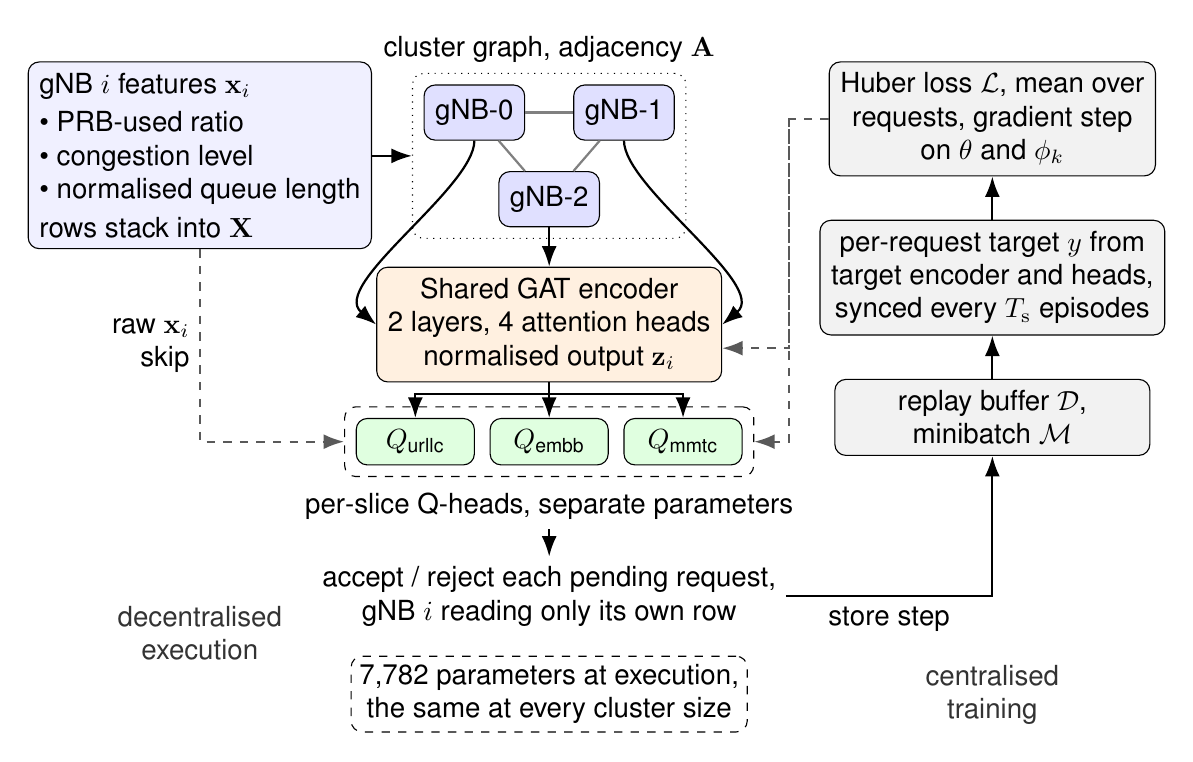
\begin{tikzpicture}[
  font=\sffamily\normalsize,
  box/.style={draw, rounded corners, minimum height=0.7cm, align=center, inner xsep=4pt, inner ysep=4pt},
  node1/.style={box, fill=blue!12, minimum width=1.0cm},
  node2/.style={box, fill=blue!12, minimum width=1.0cm},
  node3/.style={box, fill=blue!12, minimum width=1.0cm},
  encoder/.style={box, fill=orange!12, minimum width=2.6cm},
  qhead/.style={box, fill=green!12, minimum width=1.5cm, minimum height=0.55cm},
  client/.style={box, fill=violet!10, minimum width=1.8cm},
  server/.style={box, fill=orange!14, minimum width=2.0cm},
  arrow/.style={-{Latex[length=2.6mm, width=1.9mm]}, thick},
  train/.style={box, fill=gray!10, minimum width=4.0cm},
  obs/.style={box, fill=blue!6, align=left},
  dashedarrow/.style={-{Latex[length=2.6mm, width=1.9mm]}, thick, dashed},
]

% ===== AXIOM per-agent pipeline =====
% 2026-11-10: widened to the text width with context taken from Sec. 4 and Algorithm 1 only:
% the per-gNB features (left), the centralised training loop (right) and the execution label.

% 3-gNB fully-connected graph
\node[node1] (n1) at (-0.95,2.1) {gNB-0};
\node[node2] (n2) at (0.95,2.1) {gNB-1};
\node[node3] (n3) at (0,1.0) {gNB-2};
\draw[thick, gray] (n1) -- (n2);
\draw[thick, gray] (n1) -- (n3);
\draw[thick, gray] (n2) -- (n3);
\node[draw, dotted, rounded corners, fit=(n1)(n2)(n3), inner sep=4pt] (graph) {};
\node[anchor=south, font=\sffamily\normalsize] at (graph.north) {cluster graph, adjacency $\mathbf{A}$};

\node[encoder, below=0.5cm of n3] (gat) {Shared GAT encoder\\\normalsize 2 layers, 4 attention heads\\\normalsize normalised output $\mathbf{z}_i$};
\draw[arrow] (n1.south) .. controls +(0,-0.6) and +(-0.6,0.5) .. (gat.west);
\draw[arrow] (n2.south) .. controls +(0,-0.6) and +(0.6,0.5) .. (gat.east);
\draw[arrow] (n3.south) -- (gat.north);

\node[qhead, below=0.45cm of gat, xshift=-1.7cm] (q1) {$Q_{\text{urllc}}$};
\node[qhead, below=0.45cm of gat] (q2) {$Q_{\text{embb}}$};
\node[qhead, below=0.45cm of gat, xshift=1.7cm] (q3) {$Q_{\text{mmtc}}$};
\draw[arrow] (gat.south) -- ++(0,-0.15) -| (q1.north);
\draw[arrow] (gat.south) -- (q2.north);
\draw[arrow] (gat.south) -- ++(0,-0.15) -| (q3.north);
\node[draw, dashed, rounded corners, fit=(q1)(q2)(q3), inner sep=4pt] (qbox) {};
\node[below=0.08cm of qbox, font=\sffamily\normalsize] (qlab) {per-slice Q-heads, separate parameters};

\node[below=0.35cm of qlab, font=\sffamily\normalsize, align=center] (action) {accept / reject each pending request,\\ gNB $i$ reading only its own row};
\draw[arrow] (qlab.south) -- (action.north);
% figure audit: the size-invariant parameter count (m64/complexity.json and m73/complexity_n37.json, 3 to 37 gNBs)
\node[below=0.25cm of action, font=\sffamily\normalsize, align=center, draw, dashed, rounded corners, inner sep=3pt] (params) {7,782 parameters at execution,\\ the same at every cluster size};

% ----- left: what each gNB observes (Sec. 4.1)
\node[obs, anchor=north east] (x) at (-2.25,2.75) {gNB $i$ features $\mathbf{x}_i$\\[2pt]\textbullet\ PRB-used ratio\\\textbullet\ congestion level\\\textbullet\ normalised queue length\\[2pt] rows stack into $\mathbf{X}$};
\draw[arrow] (x.east |- graph.west) -- (graph.west);
% raw-feature skip into the heads: Q_k([z_i, x_i])
\draw[dashedarrow, gray!70!black] (x.south) |- node[pos=0.25, left, font=\sffamily\normalsize, align=right, text=black] {raw $\mathbf{x}_i$\\ skip} (qbox.west);
\node[anchor=north, font=\sffamily\normalsize, align=center, text=gray!40!black] at (action.west -| x.south) {decentralised\\ execution};

% ----- right: centralised training (Algorithm 1)
\node[train, anchor=north west] (loss) at (3.55,2.75) {Huber loss $\mathcal{L}$, mean over\\ requests, gradient step\\ on $\theta$ and $\phi_k$};
\node[train, below=0.55cm of loss] (tgt) {per-request target $y$ from\\ target encoder and heads,\\ synced every $T_{\mathrm{s}}$ episodes};
\node[train, below=0.55cm of tgt] (buf) {replay buffer $\mathcal{D}$,\\ minibatch $\mathcal{M}$};
\draw[arrow] (buf.north) -- (tgt.north |- buf.north) -- (tgt.south);
\draw[arrow] (tgt.north) -- (loss.south);
\draw[arrow] (action.east) -| node[pos=0.25, below, font=\sffamily\normalsize] {store step} (buf.south);
\draw[dashedarrow, gray!70!black] (loss.west) -- ++(-0.5,0) |- ([yshift=-0.3cm]gat.east);
\draw[dashedarrow, gray!70!black] (loss.west) ++(-0.5,0) |- (qbox.east);
\node[anchor=north, font=\sffamily\normalsize, align=center, text=gray!40!black] at (buf.south |- params.north) {centralised\\ training};

\end{tikzpicture}
\end{document}
